
%!TEX root=../../main.tex

%\begin{doublespace}


\chapter{Distributions of random variables}
\label{modeling}

\index{distribution!normal|(}

This chapter is currently identical to the corresponding chapter in \textit{Open Intro, 3rd ed.}.  It will be revised later to add content from medicine and biology.

%_________________
\section{Normal distribution}
\label{normalDist}

Among all the distributions we see in practice, one is overwhelmingly the most common. The symmetric, unimodal, bell curve is ubiquitous throughout statistics. Indeed it is so common, that people often know it as the \term{normal curve} or \termsub{normal distribution}{distribution!normal},\footnote{It is also introduced as the Gaussian distribution after Frederic Gauss, the first person to formalize its mathematical expression.} shown in Figure~\ref{simpleNormal}. Variables such as SAT scores and heights of US adult males closely follow the normal distribution.

\begin{figure}
\centering
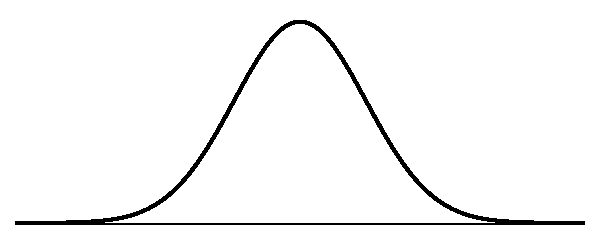
\includegraphics[width=0.7\textwidth]{ch_distributions_oi_biostat/figures/simpleNormal/simpleNormal}
\caption{A normal curve.}
\label{simpleNormal}
\end{figure}

\begin{termBox}{\tBoxTitle{Normal distribution facts}
Many variables are nearly normal, but none are exactly normal. Thus the normal distribution, while not perfect for any single problem, is very useful for a variety of problems. We will use it in data exploration and to solve important problems in statistics.\vspace{0.7mm}}
\end{termBox}


\subsection{Normal distribution model}

The normal distribution model always describes a symmetric, unimodal, bell-shaped curve. However, these curves can look different depending on the details of the model. Specifically, the normal distribution model can be adjusted using two parameters: mean and standard deviation. As you can probably guess, changing the mean shifts the bell curve to the left or right, while changing the standard deviation stretches or constricts the curve. Figure~\ref{twoSampleNormals} shows the normal distribution with mean $0$ and standard deviation $1$ in the left panel and the normal distributions with mean $19$ and standard deviation $4$ in the right panel. Figure~\ref{twoSampleNormalsStacked} shows these distributions on the same axis.

\begin{figure}[hht]
\centering
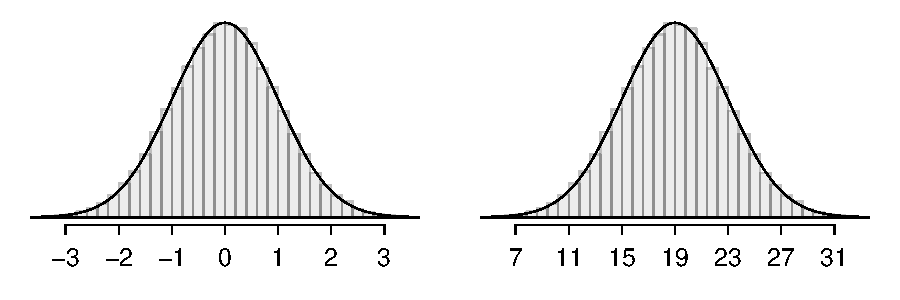
\includegraphics[width=0.85\textwidth]{ch_distributions_oi_biostat/figures/twoSampleNormals/twoSampleNormals}
\caption{Both curves represent the normal distribution, however, they differ in their center and spread. The normal distribution with mean 0 and standard deviation 1 is called the \term{standard normal distribution}.}
\label{twoSampleNormals}
\end{figure}

\begin{figure}[hht]
\centering
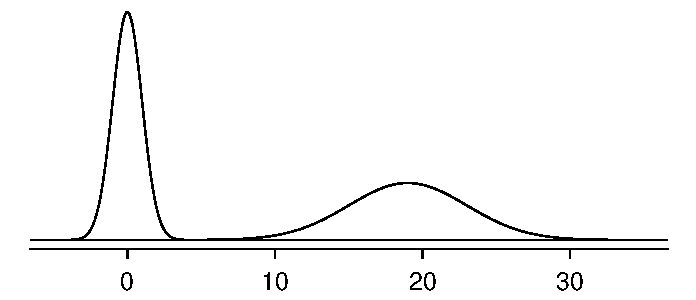
\includegraphics[width=0.6\textwidth]{ch_distributions_oi_biostat/figures/twoSampleNormalsStacked/twoSampleNormalsStacked}
\caption{The normal models shown in Figure~\ref{twoSampleNormals} but plotted together and on the same scale.}
\label{twoSampleNormalsStacked}
\end{figure}

If a normal distribution has mean $\mu$ and standard deviation $\sigma$, we may write the distribution as $N(\mu, \sigma)$\marginpar[\raggedright\vspace{-5mm}

$N(\mu, \sigma)$\vspace{1mm}\\\footnotesize Normal dist.\\with mean $\mu$\\\& st. dev. $\sigma$]{\raggedright\vspace{-5mm}

$N(\mu, \sigma)$\vspace{1mm}\\\footnotesize Normal dist.\\with mean $\mu$\\\& st. dev. $\sigma$}. The two distributions in Figure~\ref{twoSampleNormalsStacked} can be written as
\begin{align*}
N(\mu=0,\sigma=1)\quad\text{and}\quad N(\mu=19,\sigma=4)
\end{align*}
Because the mean and standard deviation describe a normal distribution exactly, they are called the distribution's \termsub{parameters}{parameter}.

\begin{exercise}
Write down the short-hand for a normal distribution with\footnote{(a)~$N(\mu=5,\sigma=3)$. (b)~$N(\mu=-100, \sigma=10)$. (c)~$N(\mu=2, \sigma=9)$.}
\begin{parts}
\item mean~5 and standard deviation~3,
\item mean~-100 and standard deviation~10, and
\item mean~2 and standard deviation~9.
\end{parts}
\end{exercise}

\subsection{Standardizing with Z-scores}

\begin{example}{Table~\vref{satACTstats} shows the mean and standard deviation for total scores on the SAT and ACT. The distribution of SAT and ACT scores are both nearly normal. Suppose Ann scored 1800 on her SAT and Tom scored 24 on his ACT. Who performed better?}\label{actSAT}
We use the standard deviation as a guide. Ann is 1 standard deviation above average on the SAT: $1500 + 300=1800$. Tom is 0.6 standard deviations above the mean on the ACT: $21+0.6\times 5=24$. In Figure~\ref{satActNormals}, we can see that Ann tends to do better with respect to everyone else than Tom did, so her score was better.
\end{example}

\begin{table}
\centering
\begin{tabular}{l r r}
  \hline
  & SAT & ACT \\
  \hline
Mean \hspace{0.3cm} & 1500 & 21 \\
SD & 300 & 5 \\
   \hline
\end{tabular}
\caption{Mean and standard deviation for the SAT and ACT.}
\label{satACTstats}
\end{table}

\begin{figure}
\centering
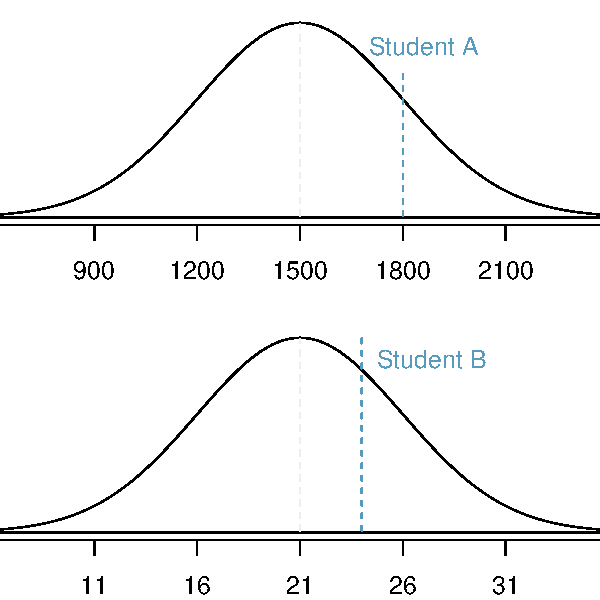
\includegraphics[width=65mm]{ch_distributions_oi_biostat/figures/satActNormals/satActNormals}
\caption{Ann's and Tom's scores shown with the distributions of SAT and ACT scores.}
\label{satActNormals}
\end{figure}

Example~\ref{actSAT} used a standardization technique called a Z-score, a method most commonly employed for nearly normal observations but that may be used with any distribution. The \term{Z-score}\marginpar[\raggedright\vspace{-3mm}

$Z$\vspace{1mm}\\\footnotesize Z-score, the\\standardized\\observation]{\raggedright\vspace{-3mm}

$Z$\vspace{1mm}\\\footnotesize Z-score, the\\standardized\\observation}\index{Z@$Z$} of an observation is defined as the number of standard deviations it falls above or below the mean. If the observation is one standard deviation above the mean, its Z-score is 1. If it is 1.5 standard deviations \emph{below} the mean, then its Z-score is -1.5. If $x$ is an observation from a distribution $N(\mu, \sigma)$, we define the Z-score mathematically as
\begin{eqnarray*}
Z = \frac{x-\mu}{\sigma}
\end{eqnarray*}
Using $\mu_{SAT}=1500$, $\sigma_{SAT}=300$, and $x_{Ann}=1800$, we find Ann's Z-score:
\begin{eqnarray*}
Z_{Ann} = \frac{x_{Ann} - \mu_{SAT}}{\sigma_{SAT}} = \frac{1800-1500}{300} = 1
\end{eqnarray*}

\begin{termBox}{\tBoxTitle{The Z-score}
The Z-score of an observation is the number of standard deviations it falls above or below the mean. We compute the Z-score for an observation $x$ that follows a distribution with mean $\mu$ and standard deviation $\sigma$ using
\begin{eqnarray*}
Z = \frac{x-\mu}{\sigma}
\end{eqnarray*}}
\end{termBox}

\begin{exercise}
Use Tom's ACT score, 24, along with the ACT mean and standard deviation to compute his Z-score.\footnote{$Z_{Tom} = \frac{x_{Tom} - \mu_{ACT}}{\sigma_{ACT}} = \frac{24 - 21}{5} = 0.6$}
\end{exercise}

Observations above the mean always have positive Z-scores while those below the mean have negative Z-scores. If an observation is equal to the mean (e.g. SAT score of 1500), then the Z-score is $0$.

\begin{exercise}
Let $X$ represent a random variable from $N(\mu=3, \sigma=2)$, and suppose we observe $x=5.19$. (a) Find the Z-score of $x$. (b) Use the Z-score to determine how many standard deviations above or below the mean $x$ falls.\footnote{(a) Its Z-score is given by $Z = \frac{x-\mu}{\sigma} = \frac{5.19 - 3}{2} = 2.19/2 = 1.095$. (b) The observation $x$ is 1.095 standard deviations \emph{above} the mean. We know it must be above the mean since $Z$ is positive.}
\end{exercise}

\begin{exercise} \label{headLZScore}
Head lengths of brushtail possums follow a nearly normal distribution with mean 92.6 mm and standard deviation 3.6 mm. Compute the Z-scores for possums with head lengths of 95.4 mm and 85.8 mm.\footnote{For $x_1=95.4$ mm: $Z_1 = \frac{x_1 - \mu}{\sigma} = \frac{95.4 - 92.6}{3.6} = 0.78$. For $x_2=85.8$ mm: $Z_2 = \frac{85.8 - 92.6}{3.6} = -1.89$.}
\end{exercise}

We can use Z-scores to roughly identify which observations are more unusual than others. One observation $x_1$ is said to be more unusual than another observation $x_2$ if the absolute value of its Z-score is larger than the absolute value of the other observation's Z-score: $|Z_1| > |Z_2|$. This technique is especially insightful when a distribution is symmetric.

\begin{exercise}
Which of the observations in Guided Practice~\ref{headLZScore} is more unusual?\footnote{Because the \emph{absolute value} of Z-score for the second observation is larger than that of the first, the second observation has a more unusual head length.}
\end{exercise}

\subsection{Normal probability table}

\begin{example}{Ann from Example~\ref{actSAT} earned a score of 1800 on her SAT with a corresponding $Z=1$. She would like to know what percentile she falls in among all SAT test-takers.}
Ann's \term{percentile} is the percentage of people who earned a lower SAT score than Ann. We shade the area representing those individuals in Figure~\ref{satBelow1800}. The total area under the normal curve is always equal to 1, and the proportion of people who scored below Ann on the SAT is equal to the \emph{area} shaded in Figure~\ref{satBelow1800}: 0.8413. In other words, Ann is in the $84^{th}$ percentile of SAT takers.
\end{example}

\begin{figure}[htb]
   \centering
   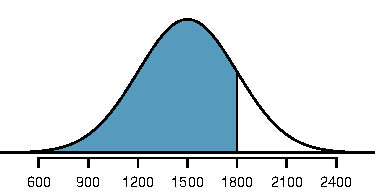
\includegraphics[width=0.6\textwidth]{ch_distributions_oi_biostat/figures/satBelow1800/satBelow1800}
   \caption{The normal model for SAT scores, shading the area of those individuals who scored below Ann.}
   \label{satBelow1800}
\end{figure}

We can use the normal model to find percentiles. A \term{normal probability table}, which lists Z-scores and corresponding percentiles, can be used to identify a percentile based on the Z-score (and vice versa). Statistical software can also be used.

A normal probability table is given in Appendix~\vref{normalProbabilityTable} and abbreviated in Table~\ref{zTableShort}. We use this table to identify the percentile corresponding to any particular Z-score. For instance, the percentile of $Z=0.43$ is shown in row $0.4$ and column $0.03$ in Table~\ref{zTableShort}: 0.6664, or the $66.64^{th}$ percentile. Generally, we round $Z$ to two decimals, identify the proper row in the normal probability table up through the first decimal, and then determine the column representing the second decimal value. The intersection of this row and column is the percentile of the observation.

\begin{figure}
\centering
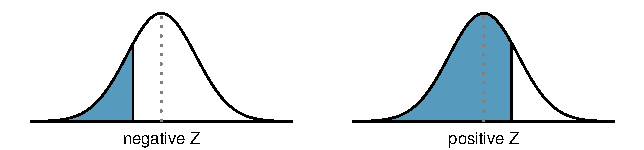
\includegraphics[width=0.9\textwidth]{ch_distributions_oi_biostat/figures/normalTails/normalTails}
\caption{The area to the left of $Z$ represents the percentile of the observation.}
\label{normalTails}
\end{figure}

\begin{table}
\centering
\begin{tabular}{c | rrrrr | rrrrr |}
  \cline{2-11}
&&&& \multicolumn{4}{c}{Second decimal place of $Z$} &&& \\
  \cline{2-11}
$Z$ & 0.00 & 0.01 & 0.02 & \highlightT{0.03} & \highlightO{0.04} & 0.05 & 0.06 & 0.07 & 0.08 & 0.09 \\
  \hline
  \hline
0.0 & \scriptsize{0.5000} & \scriptsize{0.5040} & \scriptsize{0.5080} & \scriptsize{0.5120} & \scriptsize{0.5160} & \scriptsize{0.5199} & \scriptsize{0.5239} & \scriptsize{0.5279} & \scriptsize{0.5319} & \scriptsize{0.5359} \\
  0.1 & \scriptsize{0.5398} & \scriptsize{0.5438} & \scriptsize{0.5478} & \scriptsize{0.5517} & \scriptsize{0.5557} & \scriptsize{0.5596} & \scriptsize{0.5636} & \scriptsize{0.5675} & \scriptsize{0.5714} & \scriptsize{0.5753} \\
  0.2 & \scriptsize{0.5793} & \scriptsize{0.5832} & \scriptsize{0.5871} & \scriptsize{0.5910} & \scriptsize{0.5948} & \scriptsize{0.5987} & \scriptsize{0.6026} & \scriptsize{0.6064} & \scriptsize{0.6103} & \scriptsize{0.6141} \\
%  May comment out 0.0-0.2 to make extra space. Then insert the following line:
%  $\vdots$ &   $\vdots$ &   $\vdots$ &   $\vdots$ &   $\vdots$ &   $\vdots$ &   $\vdots$ &   $\vdots$ &   $\vdots$ &   $\vdots$ &   $\vdots$ \\
  0.3 & \scriptsize{0.6179} & \scriptsize{0.6217} & \scriptsize{0.6255} & \scriptsize{0.6293} & \scriptsize{0.6331} & \scriptsize{0.6368} & \scriptsize{0.6406} & \scriptsize{0.6443} & \scriptsize{0.6480} & \scriptsize{0.6517} \\
\highlightT{0.4} & \scriptsize{0.6554} & \scriptsize{0.6591} & \scriptsize{0.6628} & \highlightT{\scriptsize{0.6664}} & \scriptsize{0.6700} & \scriptsize{0.6736} & \scriptsize{0.6772} & \scriptsize{0.6808} & \scriptsize{0.6844} & \scriptsize{0.6879} \\
  \hline
  0.5 & \scriptsize{0.6915} & \scriptsize{0.6950} & \scriptsize{0.6985} & \scriptsize{0.7019} & \scriptsize{0.7054} & \scriptsize{0.7088} & \scriptsize{0.7123} & \scriptsize{0.7157} & \scriptsize{0.7190} & \scriptsize{0.7224} \\
  0.6 & \scriptsize{0.7257} & \scriptsize{0.7291} & \scriptsize{0.7324} & \scriptsize{0.7357} & \scriptsize{0.7389} & \scriptsize{0.7422} & \scriptsize{0.7454} & \scriptsize{0.7486} & \scriptsize{0.7517} & \scriptsize{0.7549} \\
  0.7 & \scriptsize{0.7580} & \scriptsize{0.7611} & \scriptsize{0.7642} & \scriptsize{0.7673} & \scriptsize{0.7704} & \scriptsize{0.7734} & \scriptsize{0.7764} & \scriptsize{0.7794} & \scriptsize{0.7823} & \scriptsize{0.7852} \\
\highlightO{0.8} & \scriptsize{0.7881} & \scriptsize{0.7910} & \scriptsize{0.7939} & \scriptsize{0.7967} & \highlightO{\scriptsize{0.7995}} & \scriptsize{0.8023} & \scriptsize{0.8051} & \scriptsize{0.8078} & \scriptsize{0.8106} & \scriptsize{0.8133} \\
  0.9 & \scriptsize{0.8159} & \scriptsize{0.8186} & \scriptsize{0.8212} & \scriptsize{0.8238} & \scriptsize{0.8264} & \scriptsize{0.8289} & \scriptsize{0.8315} & \scriptsize{0.8340} & \scriptsize{0.8365} & \scriptsize{0.8389} \\
  \hline
  \hline
  1.0 & \scriptsize{0.8413} & \scriptsize{0.8438} & \scriptsize{0.8461} & \scriptsize{0.8485} & \scriptsize{0.8508} & \scriptsize{0.8531} & \scriptsize{0.8554} & \scriptsize{0.8577} & \scriptsize{0.8599} & \scriptsize{0.8621} \\
  1.1 & \scriptsize{0.8643} & \scriptsize{0.8665} & \scriptsize{0.8686} & \scriptsize{0.8708} & \scriptsize{0.8729} & \scriptsize{0.8749} & \scriptsize{0.8770} & \scriptsize{0.8790} & \scriptsize{0.8810} & \scriptsize{0.8830} \\
  $\vdots$ &   $\vdots$ &   $\vdots$ &   $\vdots$ &   $\vdots$ &   $\vdots$ &   $\vdots$ &   $\vdots$ &   $\vdots$ &   $\vdots$ &   $\vdots$ \\
   \hline
\end{tabular}
\caption{A section of the normal probability table. The percentile for a normal random variable with $Z=0.43$ has been \highlightT{highlighted}, and the percentile closest to 0.8000 has also been \highlightO{highlighted}.}
\label{zTableShort}
\end{table}

We can also find the Z-score associated with a percentile. For example, to identify Z for the $80^{th}$ percentile, we look for the value closest to 0.8000 in the middle portion of the table: 0.7995. We determine the Z-score for the $80^{th}$ percentile by combining the row and column Z values: 0.84.

\begin{exercise}
Determine the proportion of SAT test takers who scored better than Ann on the SAT.\footnote{If 84\% had lower scores than Ann, the number of people who had better scores must be 16\%. (Generally ties are ignored when the normal model, or any other continuous distribution, is used.)}
\end{exercise}


\textC{\newpage}


\subsection{Normal probability examples}

Cumulative SAT scores are approximated well by a normal model, $N(\mu=1500, \sigma=300)$.

\begin{example}{Shannon is a randomly selected SAT taker, and nothing is known about Shannon's SAT aptitude. What is the probability Shannon scores at least 1630 on her SATs?}\label{satAbove1630Exam}
First, always draw and label a picture of the normal distribution. (Drawings need not be exact to be useful.) We are interested in the chance she scores above 1630, so we shade this upper tail:
\begin{center}
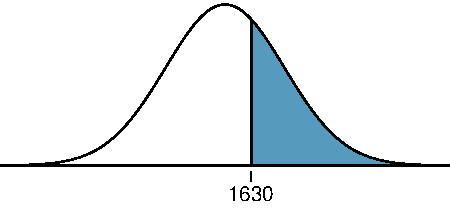
\includegraphics[width=0.45\textwidth]{ch_distributions_oi_biostat/figures/satAbove1630/satAbove1630}
\end{center}
The picture shows the mean and the values at 2 standard deviations above and below the mean. The simplest way to find the shaded area under the curve makes use of the Z-score of the cutoff value. With $\mu=1500$, $\sigma=300$, and the cutoff value $x=1630$, the Z-score is computed as
\begin{eqnarray*}
Z = \frac{x - \mu}{\sigma} = \frac{1630 - 1500}{300} = \frac{130}{300} = 0.43
\end{eqnarray*}
We look up the percentile of $Z=0.43$ in the normal probability table shown in Table~\ref{zTableShort} or in Appendix~\vref{normalProbabilityTable}, which yields 0.6664. However, the percentile describes those who had a Z-score \emph{lower} than 0.43. To find the area \emph{above} $Z=0.43$, we compute one minus the area of the lower tail:
\begin{center}
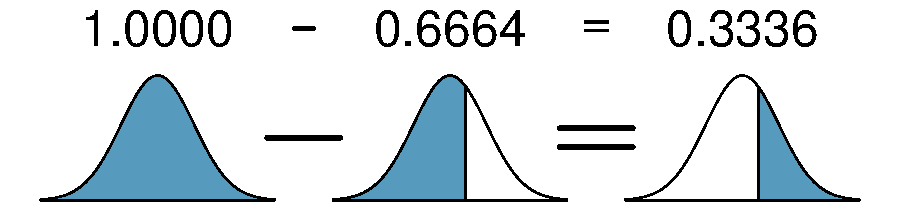
\includegraphics[width=0.5\textwidth]{ch_distributions_oi_biostat/figures/subtractingArea/subtractingArea}
\end{center}
The probability Shannon scores at least 1630 on the SAT is 0.3336.
\end{example}

\begin{tipBox}{\tipBoxTitle{always draw a picture first, and find the Z-score second}
For any normal probability situation, \emph{always always always} draw and label the normal curve and shade the area of interest first. The picture will provide an estimate of the probability. \vspace{3mm}

After drawing a figure to represent the situation, identify the Z-score for the observation of interest.\vspace{1mm}}
\end{tipBox}

\begin{exercise}
If the probability of Shannon scoring at least 1630 is 0.3336, then what is the probability she scores less than 1630? Draw the normal curve representing this exercise, shading the lower region instead of the upper one.\footnote{We found the probability in Example~\ref{satAbove1630Exam}: 0.6664. A picture for this exercise is represented by the shaded area below ``0.6664'' in Example~\ref{satAbove1630Exam}.}
\end{exercise}

\begin{example}{Edward earned a 1400 on his SAT. What is his percentile?} \label{edwardSatBelow1400}
First, a picture is needed. Edward's percentile is the proportion of people who do not get as high as a 1400. These are the scores to the left of 1400.
\begin{center}
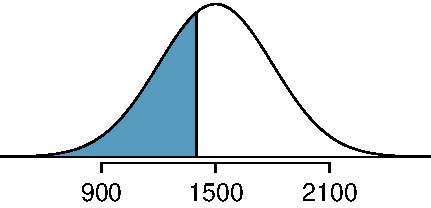
\includegraphics[width=0.4\textwidth]{ch_distributions_oi_biostat/figures/satBelow1400/satBelow1400}
\end{center}
Identifying the mean $\mu=1500$, the standard deviation $\sigma=300$, and the cutoff for the tail area $x=1400$ makes it easy to compute the Z-score:
\begin{eqnarray*}
Z = \frac{x - \mu}{\sigma} = \frac{1400 - 1500}{300} = -0.33
\end{eqnarray*}
Using the normal probability table, identify the row of $-0.3$ and column of $0.03$, which corresponds to the probability $0.3707$. Edward is at the $37^{th}$ percentile.
\end{example}

\begin{exercise}
Use the results of Example~\ref{edwardSatBelow1400} to compute the proportion of SAT takers who did better than Edward. Also draw a new picture.\footnote{If Edward did better than 37\% of SAT takers, then about 63\% must have done better than him. \\
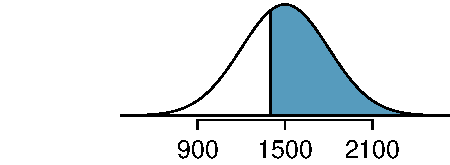
\includegraphics[height=12mm]{ch_distributions_oi_biostat/figures/satBelow1400/satAbove1400}}
\end{exercise}

\begin{tipBox}{\tipBoxTitle{areas to the right}
The normal probability table in most books gives the area to the left. If you would like the area to the right, first find the area to the left and then subtract this amount from~one.}
\end{tipBox}

\begin{exercise}
Stuart earned an SAT score of 2100. Draw a picture for each part. (a)~What is his percentile? (b)~What percent of SAT takers did better than Stuart?\footnote{Numerical answers: (a) 0.9772. (b) 0.0228.}
\end{exercise}

Based on a sample of 100 men,\footnote{This sample was taken from the USDA Food Commodity Intake Database.} the heights of male adults between the ages 20 and 62 in the US is nearly normal with mean 70.0'' and standard deviation 3.3''.

\begin{exercise}
Mike is 5'7'' and Jim is 6'4''. (a) What is Mike's height percentile? (b) What is Jim's height percentile? Also draw one picture for each~part.\footnote{First put the heights into inches: 67 and 76 inches. Figures are shown below. (a) $Z_{Mike} = \frac{67 - 70}{3.3} = -0.91\ \to\ 0.1814$. (b) $Z_{Jim} = \frac{76 - 70}{3.3} = 1.82\ \to\ 0.9656$. \\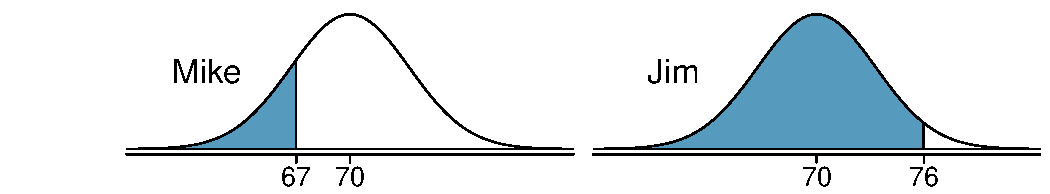
\includegraphics[height=12mm]{ch_distributions_oi_biostat/figures/mikeAndJimPercentiles/mikeAndJimPercentiles}}
\end{exercise}

The last several problems have focused on finding the probability or percentile for a particular observation. What if you would like to know the observation corresponding to a particular percentile?

\begin{example}{Erik's height is at the $40^{th}$ percentile. How tall is he?}\label{normalExam40Perc}
As always, first draw the picture.\vspace{-1mm}
\begin{center}
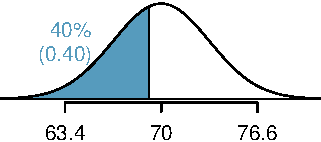
\includegraphics[width=0.35\textwidth]{ch_distributions_oi_biostat/figures/height40Perc/height40Perc}\vspace{-1mm}
\end{center}
In this case, the lower tail probability is known (0.40), which can be shaded on the diagram. We want to find the observation that corresponds to this value. As a first step in this direction, we determine the Z-score associated with the $40^{th}$ percentile.

Because the percentile is below 50\%, we know $Z$ will be negative. Looking in the negative part of the normal probability table, we search for the probability \emph{inside} the table closest to 0.4000. We find that 0.4000 falls in row $-0.2$ and between columns $0.05$ and $0.06$. Since it falls closer to $0.05$, we take this one: $Z=-0.25$.

Knowing $Z_{Erik}=-0.25$ and the population parameters $\mu=70$ and $\sigma=3.3$ inches, the Z-score formula can be set up to determine Erik's unknown height, labeled $x_{Erik}$:
\begin{eqnarray*}
-0.25 = Z_{Erik} = \frac{x_{Erik} - \mu}{\sigma} = \frac{x_{Erik} - 70}{3.3}
\end{eqnarray*}
Solving for $x_{Erik}$ yields the height 69.18 inches. That is, Erik is about 5'9'' (this is notation for 5-feet, 9-inches).
\end{example}

\begin{example}{What is the adult male height at the $82^{nd}$ percentile?}
Again, we draw the figure first.\textC{\vspace{-3mm}}
\begin{center}
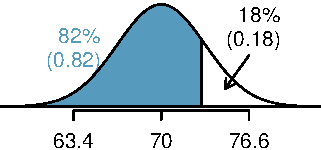
\includegraphics[width=0.28\textwidth]{ch_distributions_oi_biostat/figures/height82Perc/height82Perc}\textC{\vspace{-1mm}}
\end{center}
Next, we want to find the Z-score at the $82^{nd}$ percentile, which will be a positive value. Looking in the Z-table, we find $Z$ falls in row $0.9$ and the nearest column is $0.02$, i.e. $Z=0.92$. Finally, the height $x$ is found using the Z-score formula with the known mean $\mu$, standard deviation $\sigma$, and Z-score $Z=0.92$:
\begin{eqnarray*}
0.92 = Z = \frac{x-\mu}{\sigma} = \frac{x - 70}{3.3}
\end{eqnarray*}
This yields 73.04 inches or about 6'1'' as the height at the $82^{nd}$ percentile.
\end{example}

\begin{exercise}
(a) What is the $95^{th}$ percentile for SAT scores? (b) What is the $97.5^{th}$ percentile of the male heights? As always with normal probability problems, first draw a picture.\footnote{Remember: draw a picture first, then find the Z-score. (We leave the pictures to you.) The Z-score can be found by using the percentiles and the normal probability table. (a) We look for 0.95 in the probability portion (middle part) of the normal probability table, which leads us to row 1.6 and (about) column 0.05, i.e. $Z_{95}=1.65$. Knowing $Z_{95}=1.65$, $\mu = 1500$, and $\sigma = 300$, we setup the Z-score formula: $1.65 = \frac{x_{95} - 1500}{300}$. We solve for $x_{95}$: $x_{95} = 1995$. (b) Similarly, we find $Z_{97.5} = 1.96$, again setup the Z-score formula for the heights, and calculate $x_{97.5} = 76.5$.}
\end{exercise}

\begin{exercise}\label{more74Less69}
(a)~What is the probability that a randomly selected male adult is at least 6'2'' (74 inches)? (b)~What is the probability that a male adult is shorter than 5'9'' (69 inches)?\footnote{Numerical answers: (a) 0.1131. (b) 0.3821.}
\end{exercise}

\begin{example}{What is the probability that a random adult male is between 5'9'' and 6'2''?}
These heights correspond to 69 inches and 74 inches. First, draw the figure. The area of interest is no longer an upper or lower tail.\textC{\vspace{-2mm}}
\begin{center}
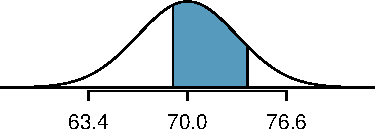
\includegraphics[width=0.35\textwidth]{ch_distributions_oi_biostat/figures/between59And62/between59And62}\textC{\vspace{-2mm}}
\end{center}
The total area under the curve is~1. If we find the area of the two tails that are not shaded (from Guided Practice~\ref{more74Less69}, these areas are $0.3821$ and $0.1131$), then we can find the middle area:\textC{\vspace{-2mm}}
\begin{center}
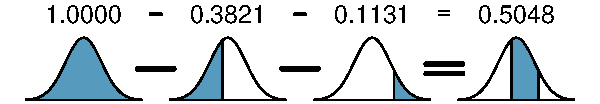
\includegraphics[width=0.6\textwidth]{ch_distributions_oi_biostat/figures/subtracting2Areas/subtracting2Areas}\textC{\vspace{-2mm}}
\end{center}
That is, the probability of being between 5'9'' and 6'2'' is 0.5048.
\end{example}

\begin{exercise}
What percent of SAT takers get between 1500 and 2000?\footnote{This is an abbreviated solution. (Be sure to draw a figure!) First find the percent who get below 1500 and the percent that get above 2000: $Z_{1500} = 0.00 \to 0.5000$ (area below), $Z_{2000} = 1.67 \to 0.0475$ (area above). Final answer: $1.0000-0.5000 - 0.0475 = 0.4525$.}
\end{exercise}

\begin{exercise}
What percent of adult males are between 5'5'' and 5'7''?\footnote{5'5'' is 65 inches. 5'7'' is 67 inches. Numerical solution: $1.000 - 0.0649 - 0.8183 = 0.1168$, i.e. 11.68\%.}
\end{exercise}


%\CalculatorVideos{calculations for the normal distribution}


\subsection{68-95-99.7 rule}

Here, we present a useful rule of thumb for the probability of falling within 1, 2, and 3 standard deviations of the mean in the normal distribution. This will be useful in a wide range of practical settings, especially when trying to make a quick estimate without a calculator or Z-table.

\begin{figure}[hht]
\centering
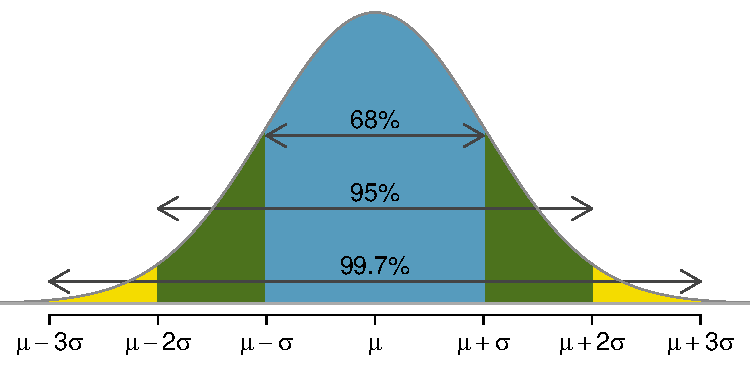
\includegraphics[height=1.9in]{ch_distributions_oi_biostat/figures/6895997/6895997}
\caption{Probabilities for falling within 1, 2, and 3 standard deviations of the mean in a normal distribution.}
\label{6895997}
\end{figure}

\begin{exercise}
Use the Z-table to confirm that about 68\%, 95\%, and 99.7\% of observations fall within 1, 2, and 3, standard deviations of the mean in the normal distribution, respectively. For instance, first find the area that falls between $Z=-1$ and $Z=1$, which should have an area of about 0.68. Similarly there should be an area of about 0.95 between $Z=-2$ and $Z=2$.\footnote{First draw the pictures. To find the area between $Z=-1$ and $Z=1$, use the normal probability table to determine the areas below $Z=-1$ and above $Z=1$. Next verify the area between $Z=-1$ and $Z=1$ is about 0.68. Repeat this for $Z=-2$ to $Z=2$ and also for $Z=-3$ to $Z=3$.}
\end{exercise}

It is possible for a normal random variable to fall 4,~5, or~even more standard deviations from the mean. However, these occurrences are very rare if the data are nearly normal. The probability of being further than 4 standard deviations from the mean is about 1-in-30,000. For 5 and 6 standard deviations, it is about 1-in-3.5 million and 1-in-1 billion, respectively.

\begin{exercise}
SAT scores closely follow the normal model with mean $\mu = 1500$ and standard deviation $\sigma = 300$. (a) About what percent of test takers score 900 to 2100? (b) What percent score between 1500 and 2100?\footnote{(a) 900 and 2100 represent two standard deviations above and below the mean, which means about 95\% of test takers will score between 900 and 2100. (b)~Since the normal model is symmetric, then half of the test takers from part~(a) ($\frac{95\%}{2} = 47.5\%$ of all test takers) will score 900 to 1500 while 47.5\% score between 1500 and 2100.}
\end{exercise}

%_________________
\section{Evaluating the normal approximation}
\label{assessingNormal}

Many processes can be well approximated by the normal distribution. We have already seen two good examples: SAT scores and the heights of US adult males. While using a normal model can be extremely convenient and helpful, it is important to remember normality is always an approximation. Testing the appropriateness of the normal assumption is a key step in many data analyses.

\index{normal probability plot|(}

Example~\ref{normalExam40Perc} suggests the distribution of heights of US males is well approximated by the normal model. We are interested in proceeding under the assumption that the data are normally distributed, but first we must check to see if this is reasonable.

There are two visual methods for checking the assumption of normality, which can be implemented and interpreted quickly. The first is a simple histogram with the best fitting normal curve overlaid on the plot, as shown in the left panel of Figure~\ref{fcidMHeights}. The sample mean $\bar{x}$ and standard deviation $s$ are used as the parameters of the best fitting normal curve. The closer this curve fits the histogram, the more reasonable the normal model assumption. Another more common method is examining a \term{normal probability plot},\footnote{Also commonly called a \term{quantile-quantile plot}.} shown in the right panel of Figure~\ref{fcidMHeights}. The closer the points are to a perfect straight line, the more confident we can be that the data follow the normal model.

\begin{figure}
\centering
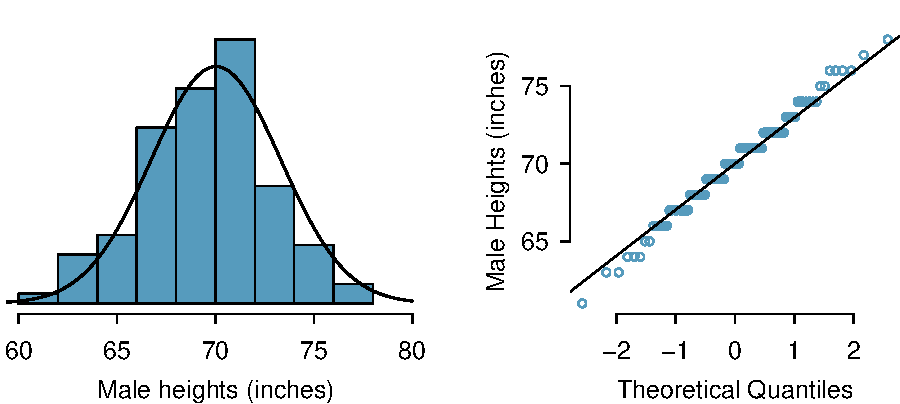
\includegraphics[width=0.8\textwidth]{ch_distributions_oi_biostat/figures/fcidMHeights/fcidMHeights}
\caption{A sample of 100 male heights. The observations are rounded to the nearest whole inch, explaining why the points appear to jump in increments in the normal probability plot.}
\label{fcidMHeights}
\end{figure}

\textC{\newpage}

\begin{example}{Three data sets of 40, 100, and 400 samples were simulated from a normal distribution, and the histograms and normal probability plots of the data sets are shown in Figure~\ref{normalExamples}. These will provide a benchmark for what to look for in plots of real data.} \label{normalExamplesExample}

\begin{figure}
\centering
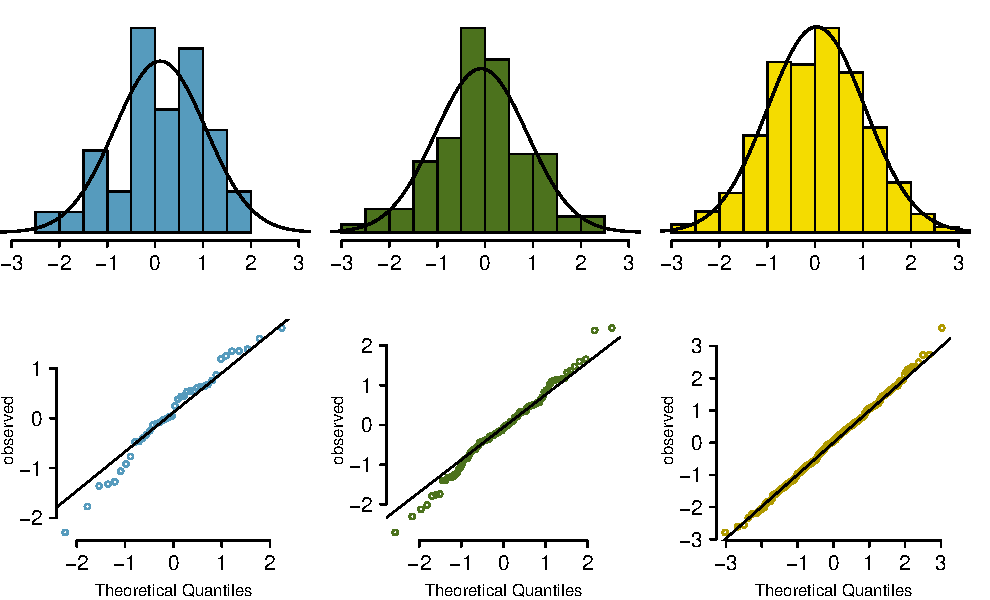
\includegraphics[width=\textwidth]{ch_distributions_oi_biostat/figures/normalExamples/normalExamples}
\caption{Histograms and normal probability plots for three simulated normal data sets; $n=40$ (left), $n=100$ (middle), $n=400$ (right).}
\label{normalExamples}
\end{figure}

The left panels show the histogram (top) and normal probability plot (bottom) for the simulated data set with 40 observations. The data set is too small to really see clear structure in the histogram. The normal probability plot also reflects this, where there are some deviations from the line. We should expect deviations of this amount for such a small data set.

The middle panels show diagnostic plots for the data set with 100 simulated observations. The histogram shows more normality and the normal probability plot shows a better fit. While there are a few observations that deviate noticeably from the line, they are not particularly extreme.

The data set with 400 observations has a histogram that greatly resembles the normal distribution, while the normal probability plot is nearly a perfect straight line. Again in the normal probability plot there is one observation (the largest) that deviates slightly from the line. If that observation had deviated 3 times further from the line, it would be of greater importance in a real data set. Apparent outliers can occur in normally distributed data but they are rare.

Notice the histograms look more normal as the sample size increases, and the normal probability plot becomes straighter and more stable.
\end{example}

\textC{\pagebreak}

\begin{example}{Are NBA player heights normally distributed? Consider all 435 NBA players from the 2008-9 season presented in Figure~\ref{nbaNormal}.\footnote{These data were collected from \oiRedirect{textbook-nba_com}{www.nba.com}.}}
We first create a histogram and normal probability plot of the NBA player heights. The histogram in the left panel is slightly left skewed, which contrasts with the symmetric normal distribution. The points in the normal probability plot do not appear to closely follow a straight line but show what appears to be a ``wave''. We can compare these characteristics to the sample of 400 normally distributed observations in Example~\ref{normalExamplesExample} and see that they represent much stronger deviations from the normal model. NBA player heights do not appear to come from a normal distribution.
\end{example}

\begin{figure}
\centering
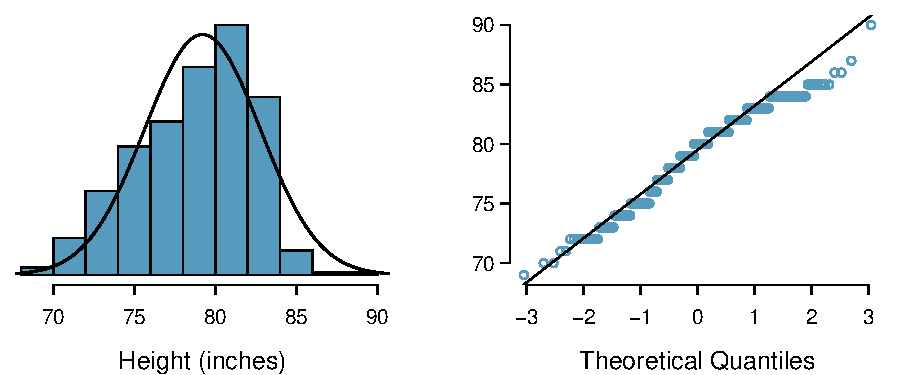
\includegraphics[width=\textwidth]{ch_distributions_oi_biostat/figures/nbaNormal/nbaNormal}
\caption{Histogram and normal probability plot for the NBA heights from the 2008-9 season.}
\label{nbaNormal}
\end{figure}

\begin{example}{Can we approximate poker winnings by a normal distribution? We consider the poker winnings of an individual over 50 days. A histogram and normal probability plot of these data are shown in Figure~\ref{pokerNormal}.}
The data are very strongly right skewed\index{skew!example: very strong} in the histogram, which corresponds to the very strong deviations on the upper right component of the normal probability plot. If we compare these results to the sample of 40 normal observations in Example~\ref{normalExamplesExample}, it is apparent that these data show very strong deviations from the normal model.
\end{example}

\begin{figure}
\centering
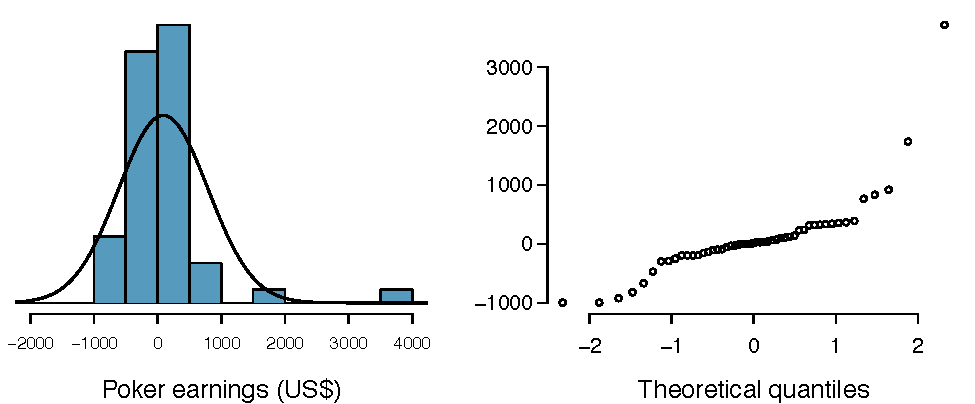
\includegraphics[width=\textwidth]{ch_distributions_oi_biostat/figures/pokerNormal/pokerNormal}
\caption{A histogram of poker data with the best fitting normal plot and a normal probability plot.}
\label{pokerNormal}
\end{figure}

\begin{exercise}\label{normalQuantileExercise}
Determine which data sets represented in Figure~\ref{normalQuantileExer} plausibly come from a nearly normal distribution. Are you confident in all of your conclusions? There are 100 (top left), 50 (top right), 500 (bottom left), and 15 points (bottom right) in the four plots.\footnote{Answers may vary a little. The top-left plot shows some deviations in the smallest values in the data set; specifically, the left tail of the data set has some outliers we should be wary of. The top-right and bottom-left plots do not show any obvious or extreme deviations from the lines for their respective sample sizes, so a normal model would be reasonable for these data sets. The bottom-right plot has a consistent curvature that suggests it is not from the normal distribution. If we examine just the vertical coordinates of these observations, we see that there is a lot of data between -20 and 0, and then about five observations scattered between 0 and 70. This describes a distribution that has a strong right skew.}
\end{exercise}

\begin{figure}
\centering
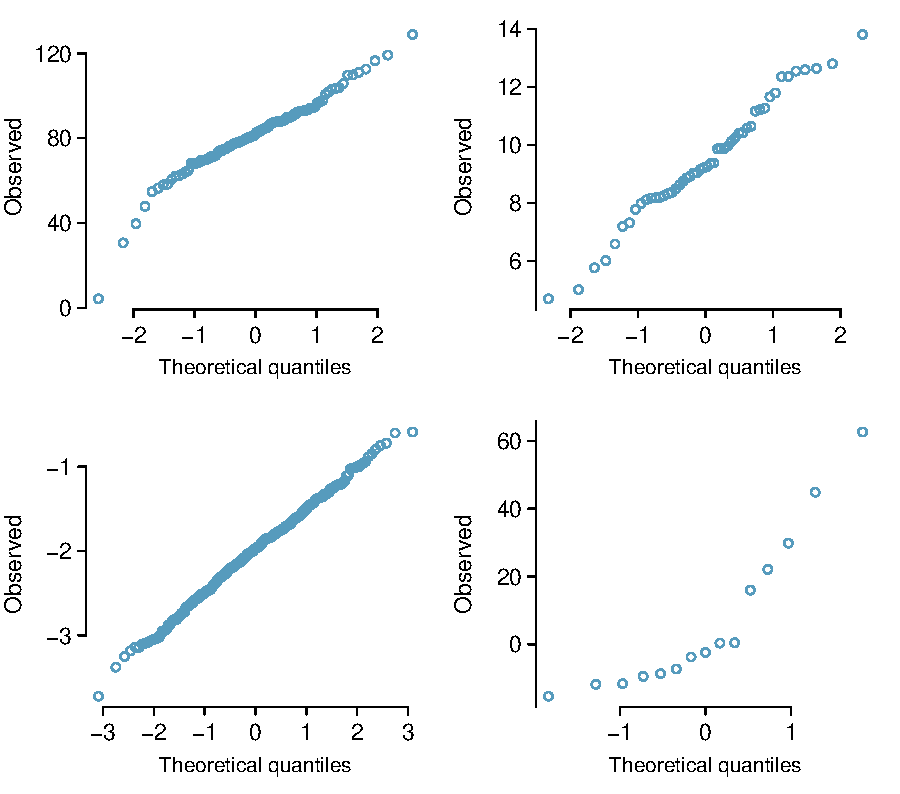
\includegraphics[width=0.9\textwidth]{ch_distributions_oi_biostat/figures/normalQuantileExer/normalQuantileExer}
\caption{Four normal probability plots for Guided Practice~\ref{normalQuantileExercise}.}
\label{normalQuantileExer}
\end{figure}

%When observations spike downwards on the left side of a normal probability plot, it means the data have more outliers in the left tail than we'd expect under a normal distribution. When observations spike upwards on the right side, it means the data have more outliers in the right tail than what we'd expect under the normal distribution.

\begin{exercise} \label{normalQuantileExerciseAdditional}
Figure~\ref{normalQuantileExerAdditional} shows normal probability plots for two distributions that are skewed. One distribution is skewed to the low end (left skewed) and the other to the high end (right skewed). Which is which?\footnote{Examine where the points fall along the vertical axis. In the first plot, most points are near the low end with fewer observations scattered along the high end; this describes a distribution that is skewed to the high end. The second plot shows the opposite features, and this distribution is skewed to the low end.}
\end{exercise}

\begin{figure}
\centering
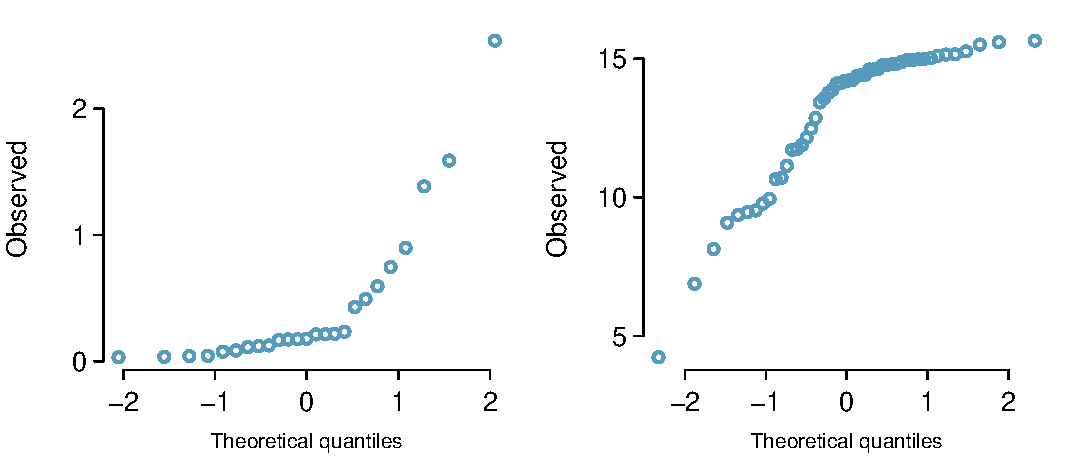
\includegraphics[width=0.9\textwidth]{ch_distributions_oi_biostat/figures/normalQuantileExer/normalQuantileExerAdditional}
\caption{Normal probability plots for Guided Practice~\ref{normalQuantileExerciseAdditional}.}
\label{normalQuantileExerAdditional}
\end{figure}


\index{normal probability plot|)}
\index{distribution!normal|)}


%_________________
\section{Geometric distribution (special topic)}
\label{geomDist}

How long should we expect to flip a coin until it turns up \resp{heads}? Or how many times should we expect to roll a die until we get a \resp{1}? These questions can be answered using the geometric distribution. We first formalize each trial -- such as a single coin flip or die toss -- using the Bernoulli distribution, and then we combine these with our tools from probability (Chapter~\ref{probability}) to construct the geometric distribution.

\subsection{Bernoulli distribution}
\label{bernoulli}

\index{distribution!Bernoulli|(}

Stanley Milgram\index{Milgram, Stanley} began a series of experiments in 1963 to estimate what proportion of people would willingly obey an authority and give severe shocks to a stranger. Milgram found that about 65\% of people would obey the authority and give such shocks. Over the years, additional research suggested this number is approximately consistent across communities and time.\footnote{Find further information on Milgram's experiment at \par \ \ \hspace{0.2mm}\ \oiRedirect{textbook-milgram}{www.cnr.berkeley.edu/ucce50/ag-labor/7article/article35.htm}.}

Each person in Milgram's experiment can be thought of as a \term{trial}. We label a person a \term{success} if she refuses to administer the worst shock. A person is labeled a \term{failure} if she administers the worst shock. Because only 35\% of individuals refused to administer the most severe shock, we denote the \term{probability of a success} with $p=0.35$. The probability of a failure is sometimes denoted with $q=1-p$.

Thus, \resp{success} or \resp{failure} is recorded for each person in the study. When an individual trial only has two possible outcomes, it is called a \termsub{Bernoulli random variable}{distribution!Bernoulli}.

\begin{termBox}{\tBoxTitle{Bernoulli random variable, descriptive}
A Bernoulli random variable has exactly two possible outcomes. We typically label one of these outcomes a ``success'' and the other outcome a ``failure''. We may also denote a success by \resp{1} and a failure by \resp{0}.}
\end{termBox}

\begin{tipBox}{\tipBoxTitle{``success'' need not be something positive}
We chose to label a person who refuses to administer the worst shock a ``success'' and all others as ``failures''. However, we could just as easily have reversed these labels. The mathematical framework we will build does not depend on which outcome is labeled a success and which a failure, as long as we are consistent.}
\end{tipBox}

Bernoulli random variables are often denoted as \resp{1} for a success and \resp{0} for a failure. In addition to being convenient in entering data, it is also mathematically handy. Suppose we observe ten trials:
\begin{center}
\resp{0} \resp{1} \resp{1} \resp{1} \resp{1} \resp{0} \resp{1} \resp{1} \resp{0} \resp{0}
\end{center}
Then the \term{sample proportion}, $\hat{p}$, is the sample mean of these observations:
\begin{eqnarray*}
\hat{p} = \frac{\text{\# of successes}}{\text{\# of trials}} = \frac{0+1+1+1+1+0+1+1+0+0}{10} = 0.6
\end{eqnarray*}%
This mathematical inquiry of Bernoulli random variables can be extended even further. Because \resp{0} and \resp{1} are numerical outcomes, we can define the {mean} and {standard deviation} of a Bernoulli random variable.\footnote{If ${p}$ is the true probability of a success, then the mean of a Bernoulli random variable $X$ is given by
\begin{align*}
\mu = E[X] &= P(X=0)\times0 + P(X=1)\times1 \\
	&= (1-p)\times0 + p\times 1 = 0+p = p
\end{align*}
Similarly, the variance of $X$ can be computed:
\begin{align*}
\sigma^2 &= {P(X=0)(0-p)^2 + P(X=1)(1-p)^2} \\
	&= {(1-p)p^2 + p(1-p)^2} = {p(1-p)}
\end{align*}
The standard deviation is $\sigma=\sqrt{p(1-p)}$.}

\begin{termBox}{\tBoxTitle{Bernoulli random variable, mathematical}
If $X$ is a random variable that takes value 1 with probability of success $p$ and 0 with probability $1-p$, then $X$ is a Bernoulli random variable with mean and standard deviation
\begin{align*}
\mu &= p
	&\sigma&= \sqrt{p(1-p)}
\end{align*}}
\end{termBox}

In general, it is useful to think about a Bernoulli random variable as a random process with only two outcomes: a success or failure. Then we build our mathematical framework using the numerical labels \resp{1} and \resp{0} for successes and failures, respectively.

\index{distribution!Bernoulli|)}

\subsection{Geometric distribution}

\index{distribution!geometric|(}

\begin{example}{Dr. Smith wants to repeat Milgram's experiments but she only wants to sample people until she finds someone who will not inflict the worst shock.\footnote{This is hypothetical since, in reality, this sort of study probably would not be permitted any longer under current ethical standards.} If the probability a person will \emph{not} give the most severe shock is still 0.35 and the subjects are independent, what are the chances that she will stop the study after the first person? The second person? The third? What about if it takes her $n-1$ individuals who will administer the worst shock before finding her first success, i.e. the first success is on the $n^{th}$ person? (If the first success is the fifth person, then we say $n=5$.)} \label{waitForShocker}
The probability of stopping after the first person is just the chance the first person will not administer the worst shock: $1-0.65=0.35$. The probability it will be the second person is
\begin{eqnarray*}
&&P(\text{second person is the first to not administer the worst shock}) \\
&&\quad = P(\text{the first will, the second won't}) = (0.65)(0.35) = 0.228
\end{eqnarray*}
Likewise, the probability it will be the third person is $(0.65)(0.65)(0.35) = 0.148$.

If the first success is on the $n^{th}$ person, then there are $n-1$ failures and finally 1 success, which corresponds to the probability $(0.65)^{n-1}(0.35)$. This is the same as $(1-0.35)^{n-1}(0.35)$.
\end{example}

Example~\ref{waitForShocker} illustrates what is called the geometric distribution, which describes the waiting time until a success for \term{independent and identically distributed (iid)} Bernoulli random variables. In this case, the \emph{independence} aspect just means the individuals in the example don't affect each other, and \emph{identical} means they each have the same probability of success.

The geometric distribution from Example~\ref{waitForShocker} is shown in Figure~\ref{geometricDist35}. In general, the probabilities for a geometric distribution decrease \term{exponentially} fast.

\begin{figure}
\centering
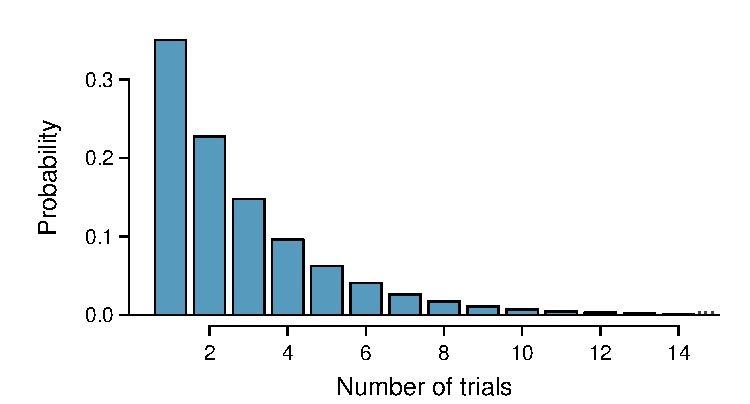
\includegraphics[width=0.8\textwidth]{ch_distributions_oi_biostat/figures/geometricDist35/geometricDist35}
\caption{The geometric distribution when the probability of success is $p=0.35$.}
\label{geometricDist35}
\end{figure}

While this text will not derive the formulas for the mean (expected) number of trials needed to find the first success or the standard deviation or variance of this distribution, we present general formulas for each.

\begin{termBox}{\tBoxTitle{Geometric Distribution\index{distribution!geometric|textbf}}
If the probability of a success in one trial is $p$ and the probability of a failure is $1-p$, then the probability of finding the first success in the $n^{th}$ trial is given by\vspace{-1.5mm}
\begin{eqnarray}
(1-p)^{n-1}p
\end{eqnarray}
The mean (i.e. expected value), variance, and standard deviation of this wait time are given by\vspace{-2.5mm}
\begin{align}
\mu &= \frac{1}{p}
	&\sigma^2&=\frac{1-p}{p^2}
	&\sigma &= \sqrt{\frac{1-p}{p^2}}
\label{geomFormulas}
\end{align}}
\end{termBox}

It is no accident that we use the symbol $\mu$ for both the mean and expected value. The mean and the expected value are one and the same.

The left side of Equation~(\ref{geomFormulas}) says that, on average, it takes $1/p$ trials to get a success. This mathematical result is consistent with what we would expect intuitively. If the probability of a success is high (e.g. 0.8), then we don't usually wait very long for a success: $1/0.8 = 1.25$ trials on average. If the probability of a success is low (e.g. 0.1), then we would expect to view many trials before we see a success: $1/0.1 = 10$ trials.

\begin{exercise}
The probability that an individual would refuse to administer the worst shock is said to be about 0.35. If we were to examine individuals until we found one that did not administer the shock, how many people should we expect to check? The first expression in Equation~(\ref{geomFormulas}) may be useful.\footnote{We would expect to see about $1/0.35 = 2.86$ individuals to find the first success.}
\end{exercise}

\begin{example}{What is the chance that Dr. Smith will find the first success within the first 4 people?} \label{marglimFirstSuccessIn4}
This is the chance it is the first ($n=1$), second ($n=2$), third ($n=3$), or fourth ($n=4$) person as the first success, which are four disjoint outcomes. Because the individuals in the sample are randomly sampled from a large population, they are independent. We compute the probability of each case and add the separate results:
\begin{eqnarray*}
&&P(n=1, 2, 3,\text{ or }4) \\
	&& \quad = P(n=1)+P(n=2)+P(n=3)+P(n=4) \\
	&& \quad = (0.65)^{1-1}(0.35) + (0.65)^{2-1}(0.35) + (0.65)^{3-1}(0.35) + (0.65)^{4-1}(0.35) \\
	&& \quad = 0.82
\end{eqnarray*}
There is an 82\% chance that she will end the study within 4~people.
\end{example}

\begin{exercise}
Determine a more clever way to solve Example~\ref{marglimFirstSuccessIn4}. Show that you get the same result.\footnote{First find the probability of the complement: $P($no success in first 4~trials$) = 0.65^4 = 0.18$. Next, compute one minus this probability: $1-P($no success in 4 trials$) = 1-0.18 = 0.82$.}
\end{exercise}

\begin{example}{Suppose in one region it was found that the proportion of people who would administer the worst shock was ``only'' 55\%. If people were randomly selected from this region, what is the expected number of people who must be checked before one was found that would be deemed a success? What is the standard deviation of this waiting time?} \label{onlyShocking55PercOfTheTimeExample}
A success is when someone will \textbf{not} inflict the worst shock, which has probability $p=1-0.55=0.45$ for this region. The expected number of people to be checked is $1/p = 1/0.45 = 2.22$ and the standard deviation is $\sqrt{(1-p)/p^2} = 1.65$.
\end{example}

\begin{exercise}
Using the results from Example~\ref{onlyShocking55PercOfTheTimeExample}, $\mu = 2.22$ and $\sigma = 1.65$, would it be appropriate to use the normal model to find what proportion of experiments would end in 3 or fewer trials?\footnote{No. The geometric distribution is always right skewed and can never be well-approximated by the normal model.}
\end{exercise}

The independence assumption is crucial to the geometric distribution's accurate description of a scenario. Mathematically, we can see that to construct the probability of the success on the $n^{th}$ trial, we had to use the Multiplication Rule for Independent Processes. It is no simple task to generalize the geometric model for dependent trials.

%\begin{exercise}
%The independence assumption is crucial to the geometric distribution's accurate description of a scenario. Why?\footnote{Independence simplified the situation. Mathematically, we can see that to construct the probability of the success on the $n^{th}$ trial, we had to use the Multiplication Rule for Independent processes. It is no simple task to generalize the geometric model for dependent trials.}
%\end{exercise}
\index{distribution!geometric|)}



\section{Binomial distribution (special topic)}
\label{binomialModel}

\index{distribution!binomial|(}

\begin{example}{Suppose we randomly selected four individuals to participate in the ``shock" study. What is the chance exactly one of them will be a success?  Let's call the four people Allen ($A$), Brittany ($B$), Caroline ($C$), and Damian ($D$) for convenience. Also, suppose 35\% of people are successes as in the previous version of this example.}\label{oneRefuser}
Let's consider a scenario where one person refuses:
\begin{eqnarray*}
&&P(A=\text{\resp{refuse}},\text{ }B=\text{\resp{shock}},\text{ }C=\text{\resp{shock}},\text{ }D=\text{\resp{shock}}) \\
 &&\quad =  P(A=\text{\resp{refuse}})\ P(B=\text{\resp{shock}})\ P(C=\text{\resp{shock}})\ P(D=\text{\resp{shock}}) \\
 &&\quad =  (0.35)  (0.65)  (0.65)  (0.65) = (0.35)^1 (0.65)^3 = 0.096
\end{eqnarray*}
But there are three other scenarios: Brittany, Caroline, or Damian could have been the one to refuse. In each of these cases, the probability is again $(0.35)^1(0.65)^3$. These four scenarios exhaust all the possible ways that exactly one of these four people could refuse to administer the most severe shock, so the total probability is $4\times(0.35)^1(0.65)^3 = 0.38$.
\end{example}

\begin{exercise}
Verify that the scenario where Brittany is the only one to refuse to give the most severe shock has probability $(0.35)^1(0.65)^3$.~\footnote{$P(A=\text{\resp{shock}},\text{ }B=\text{\resp{refuse}},\text{ }C=\text{\resp{shock}},\text{ }D=\text{\resp{shock}}) = (0.65)(0.35)(0.65)(0.65) = (0.35)^1(0.65)^3$.}
\end{exercise}

\textC{\newpage}


\subsection{The binomial distribution}

The scenario outlined in Example~\ref{oneRefuser} is a special case of what is called the binomial distribution. The \termsub{binomial distribution}{distribution!binomial} describes the probability of having exactly $k$ successes in $n$ independent Bernoulli trials with probability of a success $p$  (in Example~\ref{oneRefuser}, $n=4$, $k=1$, $p=0.35$). We would like to determine the probabilities associated with the binomial distribution more generally, i.e. we want a formula where we can use $n$, $k$, and $p$ to obtain the probability. To do this, we reexamine each part of the example.

There were four individuals who could have been the one to refuse, and each of these four scenarios had the same probability. Thus, we could identify the final probability as
\begin{eqnarray}
[\text{\# of scenarios}] \times P(\text{single scenario})
\label{genBinomialFormula}
\end{eqnarray}
The first component of this equation is the number of ways to arrange the $k=1$ successes among the $n=4$ trials. The second component is the probability of any of the four (equally probable) scenarios.

Consider $P($single scenario$)$ under the general case of $k$ successes and $n-k$ failures in the $n$ trials. In any such scenario, we apply the Multiplication Rule for independent events:
\begin{eqnarray*}
p^k(1-p)^{n-k}
\end{eqnarray*}
This is our general formula for $P($single scenario$)$.

Secondly, we introduce a general formula for the number of ways to choose $k$ successes in $n$ trials, i.e. arrange $k$ successes and $n-k$ failures:
\begin{eqnarray*}
{n\choose k} = \frac{n!}{k!(n-k)!}
\end{eqnarray*}
The quantity ${n\choose k}$ is read \term{n choose k}.\footnote{Other notation for $n$ choose $k$ includes $_nC_k$, $C_n^k$, and $C(n,k)$.} The exclamation point notation (e.g. $k!$) denotes a \term{factorial}\label{factorialDefinitionInTheBinomialSection} expression.
\begin{eqnarray*}
&& 0! = 1 \label{zeroFactorial} \\
&& 1! = 1 \\
&& 2! = 2\times1 = 2 \\
&& 3! = 3\times2\times1 = 6 \\
&& 4! = 4\times3\times2\times1 = 24 \\
&& \vdots \\
&& n! = n\times(n-1)\times...\times3\times2\times1
\end{eqnarray*}
Using the formula, we can compute the number of ways to choose $k=1$ successes in $n=4$ trials:
\begin{eqnarray*}
{4 \choose 1} = \frac{4!}{1!(4-1)!} =  \frac{4!}{1!3!} 
	= \frac{4\times3\times2\times1}{(1)(3\times2\times1)} = 4
\end{eqnarray*}
This result is exactly what we found by carefully thinking of each possible scenario in Example~\ref{oneRefuser}.

Substituting $n$ choose $k$ for the number of scenarios and $p^k(1-p)^{n-k}$ for the single scenario probability in Equation~(\ref{genBinomialFormula}) yields the general binomial formula.

\begin{termBox}{\tBoxTitle{Binomial distribution} Suppose the probability of a single trial being a success is $p$. Then the probability of observing exactly $k$ successes in $n$ independent trials is given by\vspace{-1mm}
\begin{eqnarray}
{n\choose k}p^k(1-p)^{n-k} = \frac{n!}{k!(n-k)!}p^k(1-p)^{n-k}
\label{binomialFormula}
\end{eqnarray}
Additionally, the mean, variance, and standard deviation of the number of observed successes are\vspace{-2mm}
\begin{align}
\mu &= np
	&\sigma^2 &= np(1-p)
	&\sigma &= \sqrt{np(1-p)}
\label{binomialStats}
\end{align}}
\end{termBox}

\begin{tipBox}{\tipBoxTitle{Is it binomial? Four conditions to check.\label{isItBinomialTipBox}}
(1) The trials are independent. \\
(2) The number of trials, $n$, is fixed. \\
(3) Each trial outcome can be classified as a \emph{success} or \emph{failure}. \\
(4) The probability of a success, $p$, is the same for each trial.}
\end{tipBox}

\begin{example}{What is the probability that 3 of 8 randomly selected students will refuse to administer the worst shock, i.e. 5 of 8 will?}
We would like to apply the binomial model, so we check our conditions. The number of trials is fixed ($n=8$) (condition 2) and each trial outcome can be classified as a success or failure (condition 3). Because the sample is random, the trials are independent (condition~1) and the probability of a success is the same for each trial (condition~4).

In the outcome of interest, there are $k=3$ successes in $n=8$ trials, and the probability of a success is $p=0.35$. So the probability that 3 of 8 will refuse is given by
\begin{eqnarray*}
{ 8 \choose 3}(0.35)^3(1-0.35)^{8-3}
	&=& \frac{8!}{3!(8-3)!}(0.35)^3(1-0.35)^{8-3} \\
	&=& \frac{8!}{3!5!}(0.35)^3(0.65)^5
\end{eqnarray*}
Dealing with the factorial part:
\begin{eqnarray*}
\frac{8!}{3!5!} = \frac{8\times7\times6\times5\times4\times3\times2\times1}{(3\times2\times1)(5\times4\times3\times2\times1)} = \frac{8\times7\times6}{3\times2\times1} = 56
\end{eqnarray*}
Using $(0.35)^3(0.65)^5 \approx 0.005$, the final probability is about $56*0.005 = 0.28$.
\end{example}

\begin{tipBox}{\tipBoxTitle{computing binomial probabilities}
The first step in using the binomial model is to check that the model is appropriate. The second step is to identify $n$, $p$, and $k$. The final step is to apply the formulas and interpret the results.}
\end{tipBox}

\begin{tipBox}{\tipBoxTitle{computing $n$ choose $k$}
In general, it is useful to do some cancelation in the factorials immediately. Alternatively, many computer programs and calculators have built in functions to compute $n$ choose $k$, factorials, and even entire binomial probabilities.}
\end{tipBox}

\begin{exercise}
If you ran a study and randomly sampled 40 students, how many would you expect to refuse to administer the worst shock? What is the standard deviation of the number of people who would refuse? Equation~(\ref{binomialStats}) may be useful.\footnote{We are asked to determine the expected number (the mean) and the standard deviation, both of which can be directly computed from the formulas in Equation~(\ref{binomialStats}): $\mu=np = 40\times 0.35 = 14$ and $\sigma = \sqrt{np(1-p)} = \sqrt{40\times 0.35\times 0.65} = 3.02$. Because very roughly 95\% of observations fall within 2 standard deviations of the mean (see Section~\ref{variability}), we would probably observe at least 8 but less than 20 individuals in our sample who would refuse to administer the shock.}
\end{exercise}

\begin{exercise}
The probability that a random smoker will develop a severe lung condition in his or her lifetime is about $0.3$. If you have 4 friends who smoke, are the conditions for the binomial model satisfied?\footnote{One possible answer: if the friends know each other, then the independence assumption is probably not satisfied. For example, acquaintances may have similar smoking habits.}
\end{exercise}

\begin{exercise}
\label{noMoreThanOneFriendWSevereLungCondition}%
Suppose these four friends do not know each other and we can treat them as if they were a random sample from the population. Is the binomial model appropriate? What is the probability that (a) none of them will develop a severe lung condition? (b) One will develop a severe lung condition? (c) That no more than one will develop a severe lung condition?\footnote{To check if the binomial model is appropriate, we must verify the conditions. (i) Since we are supposing we can treat the friends as a random sample, they are independent. (ii) We have a fixed number of trials ($n=4$). (iii) Each outcome is a success or failure. (iv) The probability of a success is the same for each trials since the individuals are like a random sample ($p=0.3$ if we say a ``success'' is someone getting a lung condition, a morbid choice). Compute parts (a) and (b) from the binomial formula in Equation~\eqref{binomialFormula}: $P(0) =  {4 \choose 0} (0.3)^0 (0.7)^4 = 1\times1\times0.7^4 = 0.2401$, $P(1) = {4 \choose 1} (0.3)^1(0.7)^{3} = 0.4116$. Note: $0!=1$, as shown on page~\pageref{zeroFactorial}. Part (c) can be computed as the sum of parts (a) and (b): $P(0) + P(1) = 0.2401 + 0.4116 = 0.6517$. That is, there is about a 65\% chance that no more than one of your four smoking friends will develop a severe lung condition.}
\end{exercise}

\begin{exercise}
What is the probability that at least 2 of your 4 smoking friends will develop a severe lung condition in their lifetimes?\footnote{The complement (no more than one will develop a severe lung condition) as computed in Guided Practice~\ref{noMoreThanOneFriendWSevereLungCondition} as 0.6517, so we compute one minus this value: 0.3483.}
\end{exercise}

\begin{exercise}
Suppose you have 7 friends who are smokers and they can be treated as a random sample of smokers. (a) How many would you expect to develop a severe lung condition, i.e. what is the mean? (b) What is the probability that at most 2 of your 7 friends will develop a severe lung condition.\footnote{(a)~$\mu=0.3\times7 = 2.1$. (b)~$P($0, 1, or 2 develop severe lung condition$) = P(k=0) + P(k=1)+P(k=2) = 0.6471$.}
\end{exercise}

Next we consider the first term in the binomial probability, $n$ choose $k$ under some special scenarios.

\begin{exercise}
Why is it true that ${n \choose 0}=1$ and ${n \choose n}=1$ for any number $n$?\footnote{Frame these expressions into words. How many different ways are there to arrange 0 successes and $n$ failures in $n$ trials? (1 way.) How many different ways are there to arrange $n$ successes and 0 failures in $n$ trials? (1 way.)}
\end{exercise}

\begin{exercise}
How many ways can you arrange one success and $n-1$ failures in $n$ trials? How many ways can you arrange $n-1$ successes and one failure in $n$ trials?\footnote{One success and $n-1$ failures: there are exactly $n$ unique places we can put the success, so there are $n$ ways to arrange one success and $n-1$ failures. A similar argument is used for the second question. Mathematically, we show these results by verifying the following two equations:
\begin{eqnarray*}
{n \choose 1} = n, \qquad {n \choose n-1} = n
\end{eqnarray*}}
\end{exercise}


%\CalculatorVideos{calculations for the binomial coefficient and binomial formula}




\subsection{Normal approximation to the binomial distribution}

\index{distribution!binomial!normal approximation|(}

The binomial formula is cumbersome when the sample size ($n$) is large, particularly when we consider a range of observations. In some cases we may use the normal distribution as an easier and faster way to estimate binomial probabilities.

\begin{example}{Approximately 20\% of the US population smokes cigarettes. A local government believed their community had a lower smoker rate and commissioned a survey of 400 randomly selected individuals. The survey found that only 59 of the 400 participants smoke cigarettes. If the true proportion of smokers in the community was really 20\%, what is the probability of observing 59 or fewer smokers in a sample of 400 people?}\label{exactBinomialForN400P20SmokerExample}
We leave the usual verification that the four conditions for the binomial model are valid as an exercise.

The question posed is equivalent to asking, what is the probability of observing $k=0$, 1, ..., 58, or 59 smokers in a sample of $n=400$ when $p=0.20$? We can compute these 60 different probabilities and add them together to find the answer:
\begin{align*}
&P(k=0\text{ or }k=1\text{ or }\cdots\text{ or } k=59) \\
	&\qquad= P(k=0) + P(k=1) + \cdots + P(k=59) \\
	&\qquad=0.0041
\end{align*}
If the true proportion of smokers in the community is $p=0.20$, then the probability of observing 59 or fewer smokers in a sample of $n=400$ is less than 0.0041.
\end{example}

The computations in Example~\ref{exactBinomialForN400P20SmokerExample} are tedious and long. In general, we should avoid such work if an alternative method exists that is faster, easier, and still accurate. Recall that calculating probabilities of a range of values is much easier in the normal model. We might wonder, is it reasonable to use the normal model in place of the binomial distribution? Surprisingly, yes, if certain conditions are met.

\begin{exercise}
Here we consider the binomial model when the probability of a success is $p=0.10$. Figure~\ref{fourBinomialModelsShowingApproxToNormal} shows four hollow histograms for simulated samples from the binomial distribution using four different sample sizes: $n=10, 30, 100, 300$. What happens to the shape of the distributions as the sample size increases? What distribution does the last hollow histogram resemble?\footnote{The distribution is transformed from a blocky and skewed distribution into one that rather resembles the normal distribution in last hollow histogram}
\end{exercise}

\begin{figure}[h]
\centering
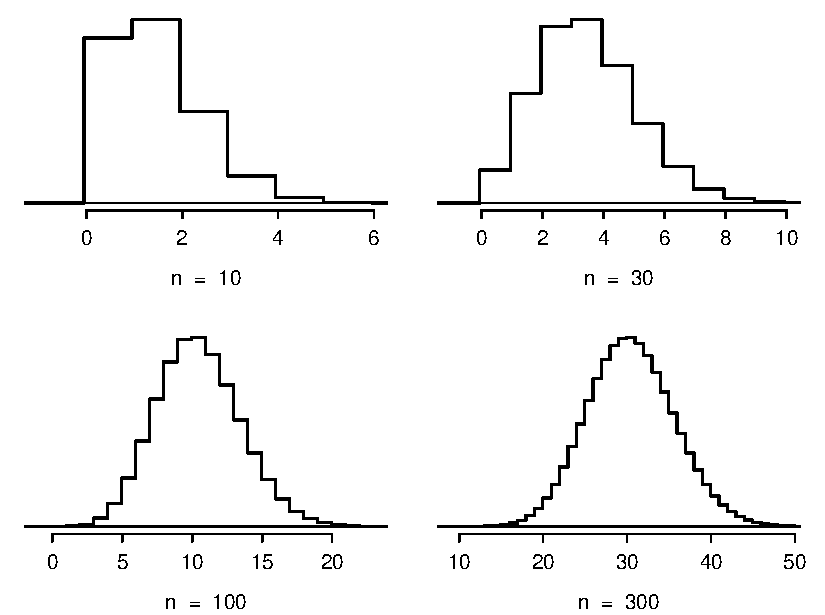
\includegraphics[width=0.92\textwidth]{ch_distributions_oi_biostat/figures/fourBinomialModelsShowingApproxToNormal/fourBinomialModelsShowingApproxToNormal}
\caption{Hollow histograms of samples from the binomial model when $p=0.10$. The sample sizes for the four plots are $n=10$, 30, 100, and 300, respectively.}
\label{fourBinomialModelsShowingApproxToNormal}
\end{figure}

\begin{termBox}{\tBoxTitle{Normal approximation of the binomial distribution}
The binomial distribution with probability of success $p$ is nearly normal when the sample size $n$ is sufficiently large that $np$ and $n(1-p)$ are both at least 10. The approximate normal distribution has parameters corresponding to the mean and standard deviation of the binomial distribution:\vspace{-1.5mm}
\begin{align*}
\mu &= np
&&\sigma= \sqrt{np(1-p)}
\end{align*}}
\end{termBox}

The normal approximation may be used when computing the range of many possible successes. For instance, we may apply the normal distribution to the setting of Example~\ref{exactBinomialForN400P20SmokerExample}.

\begin{example}{How can we use the normal approximation to estimate the probability of observing 59 or fewer smokers in a sample of 400, if the true proportion of smokers is $p=0.20$?} \label{approxBinomialForN400P20SmokerExample}
Showing that the binomial model is reasonable was a suggested exercise in Example~\ref{exactBinomialForN400P20SmokerExample}. We also verify that both $np$ and $n(1-p)$ are at least 10:
\begin{align*}
np&=400\times 0.20=80
&n(1-p)&=400\times 0.8=320
\end{align*}
With these conditions checked, we may use the normal approximation in place of the binomial distribution using the mean and standard deviation from the binomial model:
\begin{align*}
\mu &= np = 80
&\sigma &= \sqrt{np(1-p)} = 8
\end{align*}
We want to find the probability of observing fewer than 59 smokers using this model.
\end{example}

\begin{exercise}
Use the normal model $N(\mu=80, \sigma=8)$ to estimate the probability of observing fewer than 59 smokers. Your answer should be approximately equal to the solution of Example~\ref{exactBinomialForN400P20SmokerExample}: 0.0041.\footnote{Compute the Z-score first: $Z=\frac{59 - 80}{8} = -2.63$. The corresponding left tail area is 0.0043.}
\end{exercise}


\subsection{The normal approximation breaks down on small intervals}

\begin{caution}
{The normal approximation may fail on small intervals}
{The normal approximation to the binomial distribution tends to perform poorly when estimating the probability of a small range of counts, even when the conditions are met.}
\end{caution}

Suppose we wanted to compute the probability of observing 69, 70, or 71 smokers in 400 when $p=0.20$. With such a large sample, we might be tempted to apply the normal approximation and use the range 69 to 71. However, we would find that the binomial solution and the normal approximation notably differ:
\begin{align*}
\text{Binomial:}&\ 0.0703
&\text{Normal:}&\ 0.0476
\end{align*}
We can identify the cause of this discrepancy using Figure~\ref{normApproxToBinomFail}, which shows the areas representing the binomial probability (outlined) and normal approximation (shaded). Notice that the width of the area under the normal distribution is 0.5 units too slim on both sides of the interval.

\begin{figure}[h]
\centering
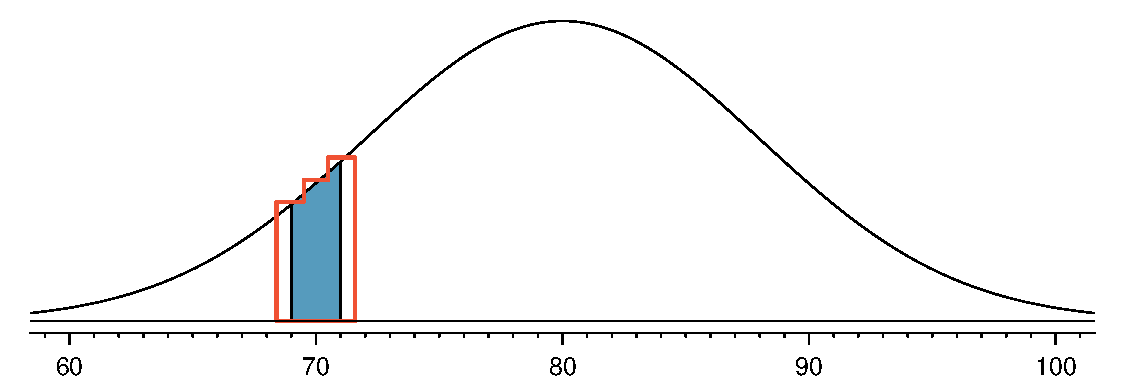
\includegraphics[width=\textwidth]{ch_distributions_oi_biostat/figures/normApproxToBinomFail/normApproxToBinomFail}
\caption{A normal curve with the area between 69 and 71 shaded. The outlined area represents the exact binomial probability.}
\label{normApproxToBinomFail}
\end{figure}

\begin{tipBox}{\tipBoxTitle{Improving the accuracy of the normal approximation to the binomial distribution}
The normal approximation to the binomial distribution for intervals of values is usually improved if cutoff values are modified slightly. The cutoff values for the lower end of a shaded region should be reduced by 0.5, and the cutoff value for the upper end should be increased by 0.5.}
\end{tipBox}

The tip to add extra area when applying the normal approximation is most often useful when examining a range of observations. While it is possible to apply it when computing a tail area, the benefit of the modification usually disappears since the total interval is typically quite wide.

\index{distribution!binomial!normal approximation|)}
\index{distribution!binomial|)}



%_________________
\section{More discrete distributions (special topic)}
\label{discreteModels}

\subsection{Negative binomial distribution}
\label{negativeBinomial}

\index{distribution!negative binomial|(}

The geometric distribution describes the probability of observing the first success on the $n^{th}$ trial. The \termsub{negative binomial distribution}{distribution!negative binomial} is more general: it describes the probability of observing the $k^{th}$ success on the $n^{th}$ trial.

\begin{example}{Each day a high school football coach tells his star kicker, Brian, that he can go home after he successfully kicks four 35 yard field goals. Suppose we say each kick has a probability $p$ of being successful. If $p$ is small -- e.g. close to 0.1 -- would we expect Brian to need many attempts before he successfully kicks his fourth field goal?}
We are waiting for the fourth success ($k=4$). If the probability of a success ($p$) is small, then the number of attempts ($n$) will probably be large. This means that Brian is more likely to need many attempts before he gets $k=4$ successes. To put this another way, the probability of $n$ being small is low.
\end{example}

To identify a negative binomial case, we check 4 conditions. The first three are common to the binomial distribution.\footnote{See a similar guide for the binomial distribution on page~\pageref{isItBinomialTipBox}.}

\begin{tipBox}{\tipBoxTitle{Is it negative binomial? Four conditions to check.}
(1) The trials are independent. \\
(2) Each trial outcome can be classified as a success or failure. \\
(3) The probability of a success ($p$) is the same for each trial. \\
(4) The last trial must be a success.}
\end{tipBox}

\begin{exercise}
Suppose Brian is very diligent in his attempts and he makes each 35 yard field goal with probability $p=0.8$. Take a guess at how many attempts he would need before making his fourth kick.\footnote{One possible answer: since he is likely to make each field goal attempt, it will take him at least 4 attempts but probably not more than 6 or 7.}
\end{exercise}

\begin{example}{In yesterday's practice, it took Brian only 6 tries to get his fourth field goal. Write out each of the possible sequence of kicks.} \label{eachSeqOfSixTriesToGetFourSuccesses}
Because it took Brian six tries to get the fourth success, we know the last kick must have been a success. That leaves three successful kicks and two unsuccessful kicks (we label these as failures) that make up the first five attempts. There are ten possible sequences of these first five kicks, which are shown in Table~\ref{successFailureOrdersForBriansFieldGoals}. If Brian achieved his fourth success ($k=4$) on his sixth attempt ($n=6$), then his order of successes and failures must be one of these ten possible sequences.

\begin{table}[ht]
\newcommand{\succObs}[1]{{\color{oiB}$\stackrel{#1}{S}$}}
\centering
\begin{tabular}{c|c ccc cl | r}
\multicolumn{8}{c}{\hspace{10mm}Kick Attempt} \\
& & 1 & 2 & 3 & 4 & \multicolumn{2}{l}{5\hfill6} \\
\hline
1&& $F$ & $F$ & \succObs{1} & \succObs{2} & \succObs{3} & \succObs{4} \\
2&& $F$ & \succObs{1} & $F$ & \succObs{2} & \succObs{3} & \succObs{4} \\
3&& $F$ & \succObs{1} & \succObs{2} & $F$ & \succObs{3} & \succObs{4} \\
4&& $F$ & \succObs{1} & \succObs{2} & \succObs{3} & $F$ & \succObs{4} \\
5&& \succObs{1} & $F$ & $F$ & \succObs{2} & \succObs{3} & \succObs{4} \\
6&& \succObs{1} & $F$ & \succObs{2} & $F$ & \succObs{3} & \succObs{4} \\
7&& \succObs{1} & $F$ & \succObs{2} & \succObs{3} & $F$ & \succObs{4} \\
8&& \succObs{1} & \succObs{2} & $F$ & $F$ & \succObs{3} & \succObs{4} \\
9&& \succObs{1} & \succObs{2} & $F$ & \succObs{3} & $F$ & \succObs{4} \\
10&& \succObs{1} & \succObs{2} & \succObs{3} & $F$ & $F$ & \succObs{4} \\
\end{tabular}
\caption{The ten possible sequences when the fourth successful kick is on the sixth attempt.}
\label{successFailureOrdersForBriansFieldGoals}
\end{table}

\end{example}

\begin{exercise} \label{probOfEachSeqOfSixTriesToGetFourSuccesses}
Each sequence in Table~\ref{successFailureOrdersForBriansFieldGoals} has exactly two failures and four successes with the last attempt always being a success. If the probability of a success is $p=0.8$, find the probability of the first sequence.\footnote{The first sequence: $0.2\times0.2\times0.8\times0.8\times0.8\times0.8 = 0.0164$.}
\end{exercise}

If the probability Brian kicks a 35 yard field goal is $p=0.8$, what is the probability it takes Brian exactly six tries to get his fourth successful kick? We can write this as
{\small\begin{align*}
&P(\text{it takes Brian six tries to make four field goals}) \\
& \quad = P(\text{Brian makes three of his first five field goals, and he makes the sixth one}) \\
& \quad = P(\text{$1^{st}$ sequence OR $2^{nd}$ sequence OR ... OR $10^{th}$ sequence})
\end{align*}
}where the sequences are from Table~\ref{successFailureOrdersForBriansFieldGoals}. We can break down this last probability into the sum of ten disjoint possibilities:
{\small\begin{align*}
&P(\text{$1^{st}$ sequence OR $2^{nd}$ sequence OR ... OR $10^{th}$ sequence}) \\
&\quad = P(\text{$1^{st}$ sequence}) + P(\text{$2^{nd}$ sequence}) + \cdots + P(\text{$10^{th}$ sequence})
\end{align*}
}The probability of the first sequence was identified in Guided Practice~\ref{probOfEachSeqOfSixTriesToGetFourSuccesses} as 0.0164, and each of the other sequences have the same probability. Since each of the ten sequence has the same probability, the total probability is ten times that of any individual sequence.

The way to compute this negative binomial probability is similar to how the binomial problems were solved in Section~\ref{binomialModel}. The probability is broken into two pieces:
\begin{align*}
&P(\text{it takes Brian six tries to make four field goals}) \\
&= [\text{Number of possible sequences}] \times P(\text{Single sequence})
\end{align*}
Each part is examined separately, then we multiply to get the final result.

We first identify the probability of a single sequence. One particular case is to first observe all the failures ($n-k$ of them) followed by the $k$ successes:
\begin{align*}
&P(\text{Single sequence}) \\
&= P(\text{$n-k$ failures and then $k$ successes}) \\
&= (1-p)^{n-k} p^{k}
\end{align*}

We must also identify the number of sequences for the general case. Above, ten sequences were identified where the fourth success came on the sixth attempt. These sequences were identified by fixing the last observation as a success and looking for all the ways to arrange the other observations. In other words, how many ways could we arrange $k-1$ successes in $n-1$ trials? This can be found using the $n$ choose $k$ coefficient but for $n-1$ and $k-1$ instead:
\begin{eqnarray*}
{n-1 \choose k-1} = \frac{(n-1)!}{(k-1)! \left((n-1) - (k-1)\right)!} = \frac{(n-1)!}{(k-1)! \left(n - k\right)!}
\end{eqnarray*}
This is the number of different ways we can order $k-1$ successes and $n-k$ failures in $n-1$ trials. If the factorial notation (the exclamation point) is unfamiliar, see page~\pageref{factorialDefinitionInTheBinomialSection}.

\begin{termBox}{\tBoxTitle{Negative binomial distribution}
The negative binomial distribution describes the probability of observing the $k^{th}$ success on the $n^{th}$ trial:
\begin{eqnarray}
P(\text{the $k^{th}$ success on the $n^{th}$ trial}) = {n-1 \choose k-1} p^{k}(1-p)^{n-k}
\label{negativeBinomialEquation}
\end{eqnarray}
where $p$ is the probability an individual trial is a success. All trials are assumed to be independent.}
\end{termBox}

\textC{\pagebreak}

\begin{example}{Show using Equation~\eqref{negativeBinomialEquation} that the probability Brian kicks his fourth successful field goal on the sixth attempt is 0.164.}
The probability of a single success is $p=0.8$, the number of successes is $k=4$, and the number of necessary attempts under this scenario is $n=6$.
\begin{align*}
{n-1 \choose k-1}p^k(1-p)^{n-k}\ 
	=\ \frac{5!}{3!2!} (0.8)^4 (0.2)^2\ 
	=\ 10\times 0.0164\ 
	=\ 0.164
\end{align*}
\end{example}

\begin{exercise}
The negative binomial distribution requires that each kick attempt by Brian is independent. Do you think it is reasonable to suggest that each of Brian's kick attempts are independent?\footnote{Answers may vary. We cannot conclusively say they are or are not independent. However, many statistical reviews of athletic performance suggests such attempts are very nearly independent.}
\end{exercise}

\begin{exercise}
Assume Brian's kick attempts are independent. What is the probability that Brian will kick his fourth field goal within 5 attempts?\footnote{If his fourth field goal ($k=4$) is within five attempts, it either took him four or five tries ($n=4$ or $n=5$). We have $p=0.8$ from earlier. Use Equation~\eqref{negativeBinomialEquation} to compute the probability of $n=4$ tries and $n=5$ tries, then add those probabilities together:
\begin{align*}
& P(n=4\text{ OR }n=5) = P(n=4) + P(n=5) \\
&\quad = {4-1 \choose 4-1} 0.8^4 + {5-1 \choose 4-1} (0.8)^4(1-0.8) = 1\times 0.41 + 4\times 0.082 = 0.41 + 0.33 = 0.74
\end{align*}}
\end{exercise}

\begin{tipBox}{\tipBoxTitle{Binomial versus negative binomial}
In the binomial case, we typically have a fixed number of trials and instead consider the number of successes. In the negative binomial case, we examine how many trials it takes to observe a fixed number of successes and require that the last observation be a success.}
\end{tipBox}

\begin{exercise}
On 70\% of days, a hospital admits at least one heart attack patient. On 30\% of the days, no heart attack patients are admitted. Identify each case below as a binomial or negative binomial case, and compute the probability.\footnote{In each part, $p=0.7$. (a) The number of days is fixed, so this is binomial. The parameters are $k=3$ and $n=7$: 0.097. (b) The last ``success'' (admitting a heart attack patient) is fixed to the last day, so we should apply the negative binomial distribution. The parameters are $k=2$, $n=4$: 0.132. (c) This problem is negative binomial with $k=1$ and $n=5$: 0.006. Note that the negative binomial case when $k=1$ is the same as using the geometric distribution.}

(a) What is the probability the hospital will admit a heart attack patient on exactly three days this week?

(b) What is the probability the second day with a heart attack patient will be the fourth day of the week?

(c) What is the probability the fifth day of next month will be the first day with a heart attack patient?
\index{distribution!negative binomial|)}
\end{exercise}


\textC{\pagebreak}


\subsection{Poisson distribution}
\label{poisson}

\index{distribution!Poisson|(}

\begin{example}{There are about 8 million individuals in New York City. How many individuals might we expect to be hospitalized for acute myocardial infarction (AMI), i.e. a heart attack, each day? According to historical records, the average number is about 4.4 individuals. However, we would also like to know the approximate distribution of counts. What would a histogram of the number of AMI occurrences each day look like if we recorded the daily counts over an entire year?} \label{amiIncidencesEachDayOver1YearInNYCExample}
A histogram of the number of occurrences of AMI on 365 days for NYC is shown in Figure~\ref{amiIncidencesOver100Days}.\footnote{These data are simulated. In practice, we should check for an association between successive days.} The sample mean (4.38) is similar to the historical average of 4.4. The sample standard deviation is about 2, and the histogram indicates that about 70\% of the data fall between 2.4 and 6.4. The distribution's shape is unimodal and skewed to the right.
\end{example}

\begin{figure}[h]
\centering
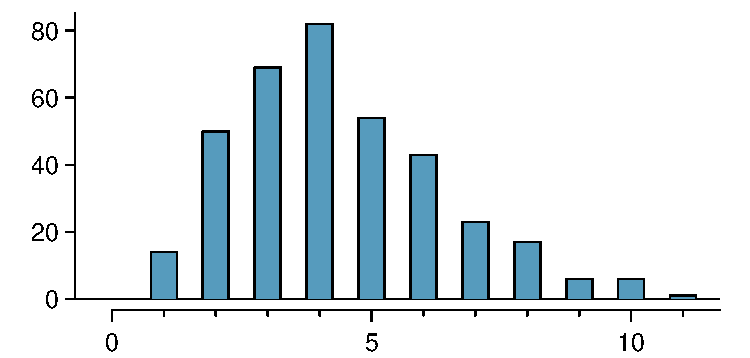
\includegraphics[width=0.7\textwidth]{ch_distributions_oi_biostat/figures/amiIncidencesOver100Days/amiIncidencesOver100Days}
\caption{A histogram of the number of occurrences of AMI on 365 separate days in NYC.}
\label{amiIncidencesOver100Days}
\end{figure}

The \termsub{Poisson distribution}{distribution!Poisson} is often useful for estimating the number of events in a large population over a unit of time. For instance, consider each of the following events:
\begin{itemize}
\setlength{\itemsep}{0mm}
\item having a heart attack,
\item getting married, and
\item getting struck by lightning.
\end{itemize}
The Poisson distribution helps us describe the number of such events that will occur in a short unit of time for a fixed population if the individuals within the population are independent.

The histogram in Figure~\ref{amiIncidencesOver100Days} approximates a Poisson distribution with rate equal to 4.4. The \term{rate} for a Poisson distribution is the average number of occurrences in a mostly-fixed population per unit of time. In Example~\ref{amiIncidencesEachDayOver1YearInNYCExample}, the time unit is a day, the population is all New York City residents, and the historical rate is 4.4. The parameter in the Poisson distribution is the rate -- or how many events we expect to observe -- and it is typically denoted by $\lambda$\marginpar[\raggedright\vspace{-5mm}

$\lambda$\vspace{0mm}\\\footnotesize Rate for the\\Poisson dist.]{\raggedright\vspace{-5mm}

$\lambda$\vspace{0mm}\\\footnotesize Rate for the\\Poisson dist.}\index{Greek!lambda@lambda ($\lambda$)}
(the Greek letter \emph{lambda})  or $\mu$. Using the rate, we can describe the probability of observing exactly $k$ events in a single unit of time.

\begin{termBox}{\tBoxTitle{Poisson distribution}
Suppose we are watching for events and the number of observed events follows a Poisson distribution with rate $\lambda$. Then
\begin{align*}
P(\text{observe $k$ events}) = \frac{\lambda^{k} e^{-\lambda}}{k!}
\end{align*}
where $k$ may take a value 0, 1, 2, and so on, and $k!$ represents $k$-factorial, as described on page~\pageref{factorialDefinitionInTheBinomialSection}. The letter $e\approx2.718$ is the base of the natural logarithm. The mean and standard deviation of this distribution are $\lambda$ and $\sqrt{\lambda}$, respectively.}
\end{termBox}

We will leave a rigorous set of conditions for the Poisson distribution to a later course. However, we offer a few simple guidelines that can be used for an initial evaluation of whether the Poisson model would be appropriate.

\begin{tipBox}{\tipBoxTitle{Is it Poisson?}
A random variable may follow a Poisson distribution if we are looking for the number of events, the population that generates such events is large, and the events occur independently of each other.}
\end{tipBox}

Even when events are not really independent -- for instance, Saturdays and Sundays are especially popular for weddings -- a Poisson model may sometimes still be reasonable if we allow it to have a different rate for different times. In the wedding example, the rate would be modeled as higher on weekends than on weekdays. The idea of modeling rates for a Poisson distribution against a second variable such as \var{dayOfTheWeek} forms the foundation of some more advanced methods that fall in the realm of \termsub{generalized linear models}{generalized linear model}. In Chapters~\ref{linRegrForTwoVar} and~\ref{multipleAndLogisticRegression}, we will discuss a foundation of linear models.

\index{distribution!Poisson|)}


%\end{doublespace}